\documentclass{article}
\usepackage[letterpaper,portrait,top=0.4in, left=0.6in, right=0.6in, bottom=1in]{geometry}

\usepackage{amsmath, amsfonts, amsthm, amssymb}
\usepackage{graphicx, float}
\usepackage{suffix}
\usepackage{esdiff}
\usepackage{multicol}
\usepackage{cancel}
\usepackage{mdframed}
\usepackage{mathtools}
\usepackage{tcolorbox}
\usepackage[colorlinks, linkcolor=blue]{hyperref}
\usepackage[per-mode=symbol]{siunitx}
\usepackage{setspace}
\usepackage{parskip}
\usepackage{enumitem}
\usepackage{titling}
\usepackage{mlmodern}

\newcommand{\alignedintertext}[1]{%
  \noalign{%
    \vtop{\hsize=\linewidth#1\par
    \expandafter}%
    \expandafter\prevdepth\the\prevdepth
  }%
}

\newcommand{\definition}[1]{\begin{tcolorbox}[colback=red!5!white,colframe=red!75!black,parbox=false] #1 \end{tcolorbox}}

\newcommand{\theorem}[2]{\begin{tcolorbox}[title={#1},colback=blue!5!white,colframe=blue!75!black,parbox=false] #2 \end{tcolorbox}}
\WithSuffix\newcommand\theorem*[1]{\begin{tcolorbox}[colback=blue!5!white,colframe=blue!75!black,parbox=false] #1 \end{tcolorbox}}

\newcommand{\example}[2]{\begin{tcolorbox}[title={Example: #1},colback=brown!5!white,colframe=brown!75!black,parbox=false] #2 \end{tcolorbox}}

\newcommand{\remark}[2]{\begin{tcolorbox}[title={#1},colback=black!5!white,colframe=black!75!black,parbox=false] #2 \end{tcolorbox}}
\WithSuffix\newcommand\remark*[1]{\begin{tcolorbox}[colback=black!5!white,colframe=black!75!black,parbox=false] #1 \end{tcolorbox}}

\newcommand*{\deriv}[1][x]{\ensuremath{\dfrac{\mathrm{d}}{\mathrm{d}#1}}}
\newcommand*{\floor}[1]{\ensuremath{\lfloor #1\rfloor}}

\title{\vspace*{-40pt}AP Physics C: Mechanics -- Class Notes}
\author{Jayden Li}
\date{\today}

\begin{document}
\setstretch{1.25}
\fontsize{11pt}{12pt}\selectfont
\setlength{\abovedisplayskip}{\abovedisplayskip/2}
\setlength{\belowdisplayskip}{\belowdisplayskip/2}
\setlength{\parindent}{0pt}
\setlength{\parskip}{2ex plus 0.5ex minus 0.2ex}
\maketitle

\tableofcontents
% \newpage

\begin{tcolorbox}[title={Summative Assessment Topics},colback=green!5!white,colframe=green!75!black,parbox=false]
	\begin{enumerate}[label={SA\arabic*.}]
		\item Honors Physics topics from summer work.
		\item \hyperref[sec:calculus]{Calculus (2)}
		\item \hyperref[sec:momentum]{Conservation of Momentum (3)}, \hyperref[sec:centerofmass]{Center of Mass (4)}, \hyperref[sec:rotation]{Rotation (5)}
	\end{enumerate}
\end{tcolorbox}


\section{Introduction}

\subsection{Jumping Monsters}

See Figure 1.1 in Notebook.

We investigate the relationship between the mass of the toy $m$ and the change in height $\Delta h$. Equipment:
\begin{itemize}
	\item Meter stick (not ruler, since ruler is only 30cm long)
	\item Phone (to record video)
	\item Balance (to measure mass in grams and kilograms, a scale measures weight in Newtons)
	\item Washers, paper clips and tape (to increase mass of toy)
\end{itemize}

We collect many data points. We will collect 5 data points, which is 5 conditions, which is 5 different masses to test.  We want to repeat every mass a few times too; we will test every mass 3 times (``3 trials''). In total, the toy will jump $5\cdot 3=15$ times. Trial means that conditions/masses are the same.

Results/data are in Table 1.2 in Notebook.

Based on conservation of energy:
\begin{equation*}
    \text{PE}_ \text{s}= \text{PE}_ \text{g}
	\implies \frac12kx^2=mgh
	\implies h=\frac{kx^2}{2mg}=\frac{kx^2}{2g}\cdot\frac1m
\end{equation*}
If we graph mass $m$ against height $\Delta h$, this is an inverse relationship, as $kx^2/2g$ is a constant (the spring distance $x$ does not change for one toy, $k$ is spring constant, and $g$ is acceleration due to gravity).

Because we want a linear relationship, we can graph inverse mass $1/m$ against height $\Delta h$. This becomes a line with slope $kx^2/2g$.

Logger pro graph, plotting inverse mass in $1/\text{kg}$ against height in meters:

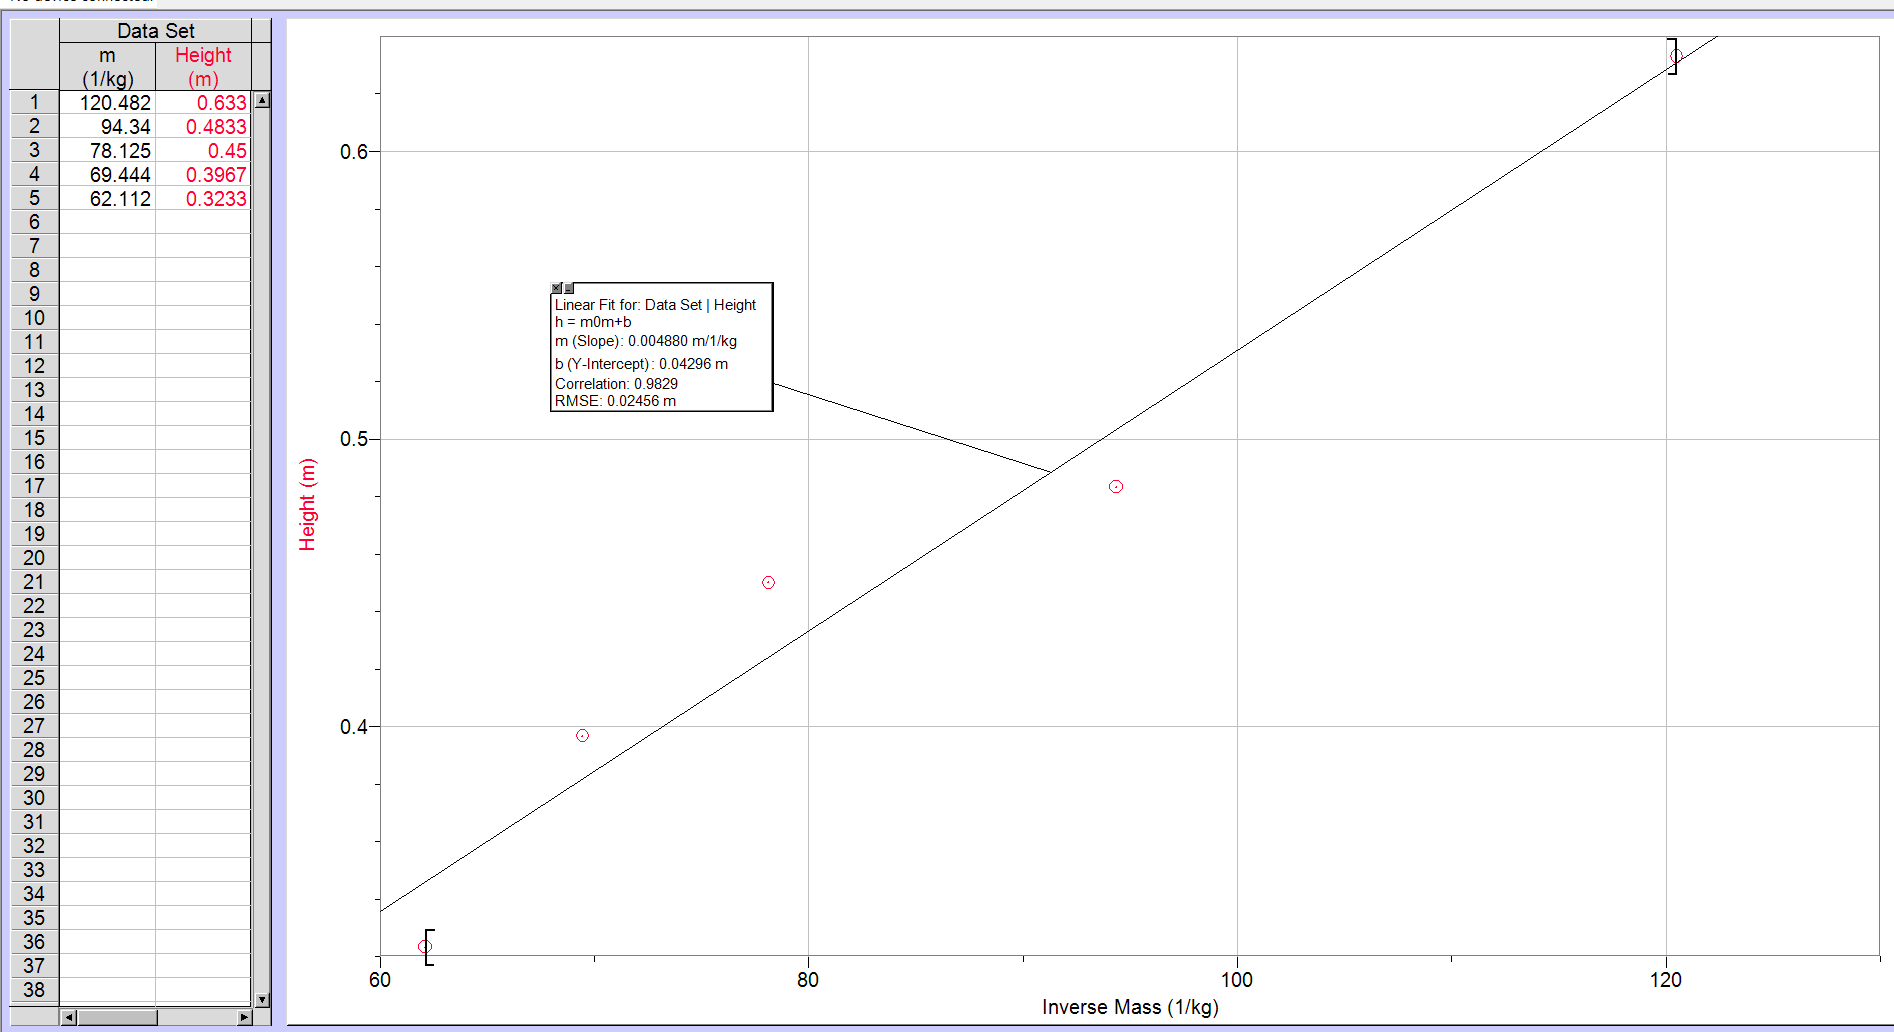
\includegraphics[width=\linewidth]{loggerpro0903.png}
\begin{equation*}
	\text{Slope}
	=m 
	=\frac{kx^2}{2g}
	=0.004880
	\implies k=m\cdot \frac{2g}{x^2}
	=0.004880\cdot \frac{2(9.81)}{(1.5/100)^2}
	=\boxed{425.536\,\si{\newton\per\meter}}
\end{equation*}

\remark{Linearization}{Linearization is a powerful technique. For example, with Kepler's third law of planetary motion:
\begin{equation*}
    \frac{T^2}{r^3}=\frac{4\pi^2}{GM}
\end{equation*}
is annoying to plot when we plot $T$ against $r$. We rearrange and plot $T^2$ against $r^3$ for a linear relationship:
\begin{equation*}
    T^2=\frac{4\pi^2}{GM}r^3
\end{equation*}
$4\pi^2/GM$ is a constant/the slope. We take $y=T^2$ and $x=r^3$, and we have the fitted slope $m=4\pi^2/GM$.}

\subsection{Projectile Motion}

Two-dimensional motion, $x$ and $y$-directions. The type of motion in the two directions are different.

$x$-direction has constant velocity because there is no net force and no acceleration acting in the $x$-direction.
\begin{equation*}
    v_x=\frac{\Delta x}{\Delta t}
	\iff \Delta x=v_x(\Delta t)
\end{equation*}

$y$-direction has constant acceleration due to gravity $-g$.
\begin{align*}
	v_y&=v_{0y}+at \\
	\Delta y&=v_{0y}t+\frac12at^2 \\
	v_y^2&=v+{0y}^2+2a\Delta y
\end{align*}

\subsubsection{Special cases}

In horizontal projectile motion, $v_{0y}=0\,\si{\meter\per\second}$.

When the projectile reaches its highest point in general 2-dimensional motion, then at the highest point, there is no $y$-velocity: $v_y=0\,\si{\meter\per\second}$.

If the projectile is launched at a certain velocity $v_0$ at an angle $\theta$, we have initial $x$ and initial $y$-velocities:
\begin{align*}
	v_x=v_{0x}&=v_0\cos\theta \\
	v_{0y}&=v_0\sin\theta
\end{align*}

\subsection{Momentum Lab}

Equipment:
\begin{itemize}
	\item Motion sensor/detector
	\item Force sensor: measures force
	\item Cart connected to plunger; plunger is a metal rod with a spring inside
\end{itemize}

Push cart on a track, measure force and velocity to obtain the mass of the cart. To improve the accuracy and lower the percent error:
\begin{itemize}
	\item Check if the track is level, if the track is inclined then the cart is not moving at a constant velocity (disregarding friction) before and after the collision.
	\item Reduce friction
	\item Increase the number of \textbf{experimental conditions} (cannot increase the number of trials, because trial has the same conditions like initial speed, which is not possible to make sure) by pushing it more times
	\item Line up force sensor and cart/track
\end{itemize}

\subsection{AP Formula Sheet}

$G$ universal gravitational constant is important. We should take acceleration due to gravity on Earth $g=10\,\si{\meter\per\second\squared}$. Magnitude of gravitational field of earth is also $g=10\,\si{\newton\per\kilo\gram}$. These units are equivalent.

Kinematic equations for \textbf{constant acceleration} and therefore constant force:
\begin{equation*}
    \Delta x=v_0t+\frac12at^2 \qquad
	v=v_0+at \qquad
	v^2=v_0^2+2a\Delta x
\end{equation*}
Newton's second law does not have to be complicated; $\Sigma F=ma$ is fine.

Maximum friction $\lVert \vec{F}_f \rVert =\lVert \mu \vec{F}_N \rVert $ tells us, where $\vec{F}_N$ is normal force:
\begin{itemize}
	\item kinetic friction $\vec{F}_k=\mu_k \vec{F}_N$
	\item Maximum static friction $\vec{F}_\text{s,max}=\mu_\text{s,max}\vec{F}_N$
	\item Static friction $\lVert \vec{F}_\text{s} \rVert <\vec{F}_\text{s,max}$.
\end{itemize}

\section{Calculus}
\label{sec:calculus}

\subsection{Calculus-Based Equations}

\theorem{Kinematics}{
	\begin{alignat*}{2}
		v&=\diff xt &\qquad \Delta x=\int v\,\mathrm{d}t \\
		a&=\diff vt=\diff[2]{x}{t} &\qquad \Delta v=\int a\,\mathrm{d}t
	\end{alignat*}
	where $x$ is position, $v$ is velocity and $a$ is acceleration. These will apply to all situations (for constant velocity, constant acceleration or nonconstant acceleration).
}

Integrate with respect to independent variable; integrand is dependent variable. See Figure 2.1.

\theorem{Connecting dynamics/forces and kinematics}{
Newton's second law: $\Sigma F=ma$. Acceleration $a$ connects forces and dynamics to kinematics.

Suppose we are given position $x$. Then we can calculate the acceleration by differentiation:
\begin{equation*}
	a=\diff[2]xt
	\implies F=ma=m\diff[2]xt
\end{equation*}
}

Connecting energy and kinematics by kinetic energy $K=mv^2/2$.

\theorem{Work and force-position graphs}{
	Consider a force-position graph (Figure 2.2). The area under the curve is the work done, or change in energy: $W=\Delta E$. The relationship is as follows, where $\Sigma F$ is the net force:
	\begin{equation*}
	    \Delta E=\int\Sigma  F\,\mathrm{d}x
		\qquad \Sigma F=\diff Ex
	\end{equation*}
}

\theorem{Power and time}{
	Power is the rate of change of energy with respect to time:
	\begin{equation*}
		\Delta E=\int P\,\mathrm{d}t \qquad P=\diff Et
	\end{equation*}
	The change in energy is the area under the curve of a power-time graph (Figure 3.3).
}

\theorem{Force and time}{
	Recall that for constant net force $\Sigma F$, impulse $J=\Delta p=\Sigma F\cdot \Delta t$. For a force-time graph in Figure 2.4:
	\begin{equation*}
	    J=\Delta p=\int F\,\mathrm{d}t
		\qquad 
		F=\diff{p}{t}=m\cdot \diff vt=ma
	\end{equation*}
	(Impulse $\Delta p=I=J=\Delta(mv)=m \cdot \Delta v$, since mass usually does not change. $\mathrm{d}p=F\mathrm{d} t \implies \mathrm{d}(mv)=m\mathrm{d} v=F\mathrm{d} t\implies F=m(\mathrm{d}v/\mathrm{d}t)=ma$)
}

\theorem{Rotational kinematics}{
	\begin{equation*}
		\omega=\diff{\theta}t \qquad
		\alpha=\diff{\omega}{t} \qquad
		\Delta\theta=\int \omega\,\mathrm{d}t \qquad
		\Delta \omega=\int \alpha\,\mathrm{d}t
	\end{equation*}
}

\subsection{Potential Energy}

Suppose we drop a ball from a certain height. We know that the work done by the force of gravity is positive work, but since energy is conserved, the potential energy in the ball must decrease. Therefore, we have:
\begin{equation*}
    -W=\Delta U 
\end{equation*}
But, we know that work is force times distance:
\begin{equation*}
	\Delta U=-F_y\cdot \Delta y
	\implies F_y=-\frac{\Delta U}{\Delta y}
\end{equation*}
where $\Delta y$ is the distance the ball is dropped, or the distance over which the force acts. By black magic, we can change this into a derivative:
\begin{equation*}
	F_y=-\diff Uy
\end{equation*}
Must have negative sign. So, we can also have potential energy in terms of force:
\begin{equation*}
    F_y=-\diff Uy
	\implies -F_y \,\mathrm{d}y=\mathrm{d}U
	\implies \Delta U=-\int F_y\,\mathrm{d}y
\end{equation*}
\remark*{In nature, objects want to lower their potential energy. (NOTE: lower the number, NOT the magnitude of kinetic energy.)}

\theorem{Potential energy}{
	The relationship between potential energy and force is, where $x$ is position:
	\begin{equation*}
	    \Delta U_x=-\int F_x\,\mathrm{d}x
		\qquad
		F_x=-\diff Ux
	\end{equation*}
}

In simple harmonic motion, the potential energy-displacement from equilibrium graph is a positive parabola passing through the origin. There is no potential energy at equilibrium ($x=0$) and potential energy is maximized at the highest displacement.

Total energy is the sum of kinetic energy and potential energy: $K+U$. By conservation of energy, the total energy is constant for all displacement.

\definition{The work done by a \textbf{conservative force} only depends on the initial and final position of the object, not on the path taken.}

A lot of forces are path-dependent. For example, friction depends on the length of the path, so it is not conservative. Forces associated with change in potential energy are conservative.

\example{Gravitional potential}{
	Change in gravitational potential energy is $\Delta U_g=mgy$. We can calculate the force:
	\begin{equation*}
		F_g=-\diff{U_g}{y}=-\deriv[y](mgy)=-mg
	\end{equation*}
	is consistent with the result we get from $F=ma$.
}

\example{Spring potential}{
	Change in spring potential is $U_s=kx^2/2$:
	\begin{equation*}
		F_s=-\diff{U_s}{x}=-\deriv[x]\left(\frac12kx^2\right)=-kx
	\end{equation*}
}

\subsection{Springs}

Formulas like $F_s=-kx$ and $U_s=kx^2/2$ depend on a \textbf{perfect, ideal spring}, which requires some assumptions.
\begin{itemize}
	\item The mass of the spring itself is negligible; the mass of the system is exactly the mass of the object attachde to the spring.
	\item Force exerted is $F_s=-kx$: force-displacement graph is linear and passes through the origin. From this, formula for kinetic energy follows: $U_s=-\int F_s\,\mathrm{d}x=-\int -kx\,\mathrm{d}x=kx^2/2$.
	\item No internal friction and losses. If there are, \textit{damping} occurs. This is drawn in Figure 2.5. Even though the period does not change, each successive crest and trough decreases in magnitude.
\end{itemize}

Figure 2.6 shows the energy position graph of an ideal spring. By conservation of energy, total energy $\text{TE}=U_s+K$.

Real springs are non-ideal.

\section{Conservation of Momentum}
\label{sec:momentum}

\subsection{Explosions}

\definition{An explosion is when two objects separate after being together.}

Cart of mass $m_1$ and mass $m_2$ separate after a compressed spring between them, and they move at velocity $v_1$ and $v_2$. $m_1>m_2$. By conservation of momentum:
\begin{equation*}
    m_1v_1=m_2v_2
	\implies v_2=\frac{m_1v_1}{m_2}
\end{equation*}
We calculate each object's kinetic energy:
\begin{align*}
	K_1&=\frac12m_1v_1^2 \\
	K_2&=\frac12m_2v_2^2
	   =\frac12m_2 \left( \frac{m_1v_1}{m_2} \right)^2
	   =\frac12 m_1\left(\frac{m_1}{m_2}\right)v_1^2
	   =\frac{m_1}{m_2}K_1
\end{align*}
Since $m_1>m_2$: $m_1/m_2>1\implies K_2>K_1$

\theorem*{If momentum is conserved after a collision or explosion, then the object with the lower mass (and therefore higher velocity) has higher kinetic energy.}

\subsection{Elastic Head-On Collisions}

\definition{In a head-on collisions, both objects are moving in a straight line. In a glancing collision, objects will go in different angles after the collision.}

Suppose that two objects collide head on. The objects are initially traveling at velocities $v_1,v_2$, and have velocities $v_1',v_2'$ after the collision.

By conservation of momentum and conservation of kinetic energy (because collision is elastic):
\begin{align*}
	\Sigma p&=\Sigma p' \\
	m_1v_1+m_2v_2&=m_1(v_1')+m_2(v_2') \tag{1} \\
	\frac12m_1v_1^2+\frac12m_2v_2^2&=\frac12m_1(v_1')^2+\frac12m_2(v_2')^2 \tag{2}
\end{align*}
We can use this to derive another equation:
\begin{align*}
	(2)
	&\implies \frac12m_1v_1^2+\frac12m_2v_2^2=\frac12m_1(v_1')^2+\frac12m_2(v_2')^2
	\implies m_1v_1^2+m_2v_2^2=m_1(v_1')^2+m_2(v_2')^2 \\
	&\implies m_1 v_1^2-m_1(v_1')^2=m_2(v_2')^2-m_2v_2^2
	\implies m_1 \left( v_1^2-(v_1')^2 \right)=m_2 \left( (v_2')^2-v_2^2 \right) \\
	&\implies m_1(v_1+v_1')(v_1-v_1')=m_2(v_2'+v_2)(v_2'-v_2) \\
	(1)
	&\implies m_1v_1-m_1(v_1')=m_2(v_2')-m_2v_2
	\implies m_1 \left( v_1-v_1' \right)=m_2 \left( v_2'-v_2 \right) \\
	\frac{(2)}{(1)}
	&\implies \frac{\bcancel{m_1}(v_1+v_1')(\cancel{v_1-v_1'})}{\bcancel{m_1}(\cancel{v_1-v_1'})}=\frac{\bcancel{m_2}(v_2'+v_2)(\cancel{v_2'-v_2})}{\bcancel{m_2}(\cancel{v_2'-v_2})}
	\implies v_1+v_1'=v_2+v_2'
\end{align*}

\theorem{Equations for a head-on elastic collision}{
	\begin{align*}
		m_1v_1+m_2v_2&=m_1(v_1')+m_2(v_2') \tag{Conservation of Momentum} \\
		\frac12m_1v_1^2+\frac12m_2v_2^2&=\frac12m_1(v_1')^2+\frac12m_2(v_2')^2 \tag{Conservation of Kinetic Energy} \\
		v_1+v_1'&=v_2+v_2'
	\end{align*}
}

\subsection{Ballistic Pendulum}

Bullet of mass $m$ into a block of mass $M$ at velocity $v$. The bullet lodges into the mass and travels with the block. This is a completely inelastic collision.

We can calculate the final velocity of the block by conservation of momentum $mv=(M+m)V$. From $V$ we can calculate the kinetic energy $K$, and gravitational potential energy when the block is shot is $0$. So the total mechanical energy is $K+0=K$.

The highest point in the pendulum is reached when the gravitational potential energy equals the total energy:
\begin{equation*}
	\frac12(\cancel{M+m})V^2=(\cancel{M+m})g\Delta h
	\implies \Delta h=\frac{V^2}{2g}
\end{equation*}

\subsection*{Free Response Questions}

\remark{Free response}{\begin{itemize}
	\item Use pencil or black/blue pen.
	\item Start by writing known equation.
	\item Substitution (substitute numbers with no units).
	\item Final answer clearly indicated such as \boxed{\text{boxed}}.
		\begin{itemize}
			\item If numerical, do not keep infinite number of significant figures: no square root, fraction, constants; \textbf{always 2 or 3 significant figures, never 1 s.f.!!!!!}
			\item If symbolic, leave square roots, fractions, constants:
		\end{itemize}
	\item Graphing: label axes with units:
		\begin{itemize}
			\item Name of graph is ``[value on $y$ axis] vs [value on $x$ axis]'' or ``[value on $y$] wrt [value on $x$]''.
			\item Line of best fit: equal number of points above and below the line.
			\item When determining slope of line of best fit, do not choose original values: $\text{Slope}=\Delta y/\Delta x=(y_1-y_0)/(x_1-x_0)$. \textbf{The slope has units.}
		\end{itemize}
	\item Integrals: must have limits of integration and differential.
\end{itemize}}

\subsection{Equilibrium}

\begin{itemize}
	\item In stable equilibrium, when a small external force is exerted, the object will move, and when the external force is removed, the system will return to its equilibrium position.
	\item In unstable equilibrium, the system will not return to equilibrium when the external force is removed.
	\item In neutral equilibrium, the object remains at the new location after the external force is removed.
\end{itemize}

\section{Center of Mass}
\label{sec:centerofmass}

\definition{The \textbf{center of mass} of a system is the average location of mass of a system or object. If the system/object is in a gravitational field then this is also called the center of gravity because we consider that is where the force of gravity/weight acts on the system.}

\begin{itemize}
	\item Object will rotate around its center of mass if force is applied
	\item If a normal force/support is applied at its center of mass, it will balance.
	\item The center of mass will change if the object's mass distribution changes.
	\item A system can be modeled as a single object located at the system's center of mass.
	\item If an object is symmetrical, then the center of mass is on a line of symmetry.
\end{itemize}

\theorem{Center of mass of system of particles}{The center of mass of a system of particles $( x_\text{cm}, y_\text{cm})$, each particle having mass $m_i$ and location $(x_i,y_1)$ is:
\begin{equation*}
     x_\text{cm}=\frac{\sum m_ix_i}{\sum m_i}
	\qquad  y_\text{cm}=\frac{\sum m_i y_i}{\sum m_i}
\end{equation*}
If we are asked to calculate the center of mass of a shape, we can try to reduce the shape into particles, and use these equations. These equations for $ x_\text{cm}, y_\text{cm}$ can be extended to any number of dimensions.}

As with torque, the reference point from which positions $x_i$ are measured is completely arbitrary.

The velocity of the whole system (from the center of mass position) is:
\begin{equation*}
	 v_\text{cm}
	=\diff{ x_\text{cm}}{t}
	=\deriv[t] \frac{\sum m_ix_i}{\sum m_i}
	=\frac{\sum m_i \diff{x_i}{t}}{M}
	=\boxed{\frac{\sum m_i v_i}{M}}
	\implies M v_\text{cm}=\boxed{p_\text{cm}=\sum m_iv_i} \\
\end{equation*}
The velocity of the center of mass is a weighted average of the velocities of the objects that make up the system. The momentum of the system at the center of mass is the sum of the momenta of each object in the system, of which the center of mass is measured.
\begin{equation*}
	a_\text{cm}
	=\diff[2]{ x_\text{cm}}{t}
	=\frac{\sum m_ia_i}{\sum m_i}
	=\frac{\sum F}{M}
	\implies \boxed{\Sigma F=Ma_\text{cm}}
\end{equation*}
Is Newton's second law for the center of mass.

\theorem{Center of mass, velocity, acceleration, momentum and force}{
	\begin{align*}
		v_\text{cm}&=\diff{x_\text{cm}}{t}=\frac{\sum m_iv_i}{\sum m_i}=\frac{\sum p_i}{M} \\
		p_\text{cm}&=\sum m_iv_i=\sum p_i \\
		a_\text{cm}&=\diff{v_\text{cm}}{t}=\frac{\sum m_ia_i}{\sum m_i}=\frac{\sum F_i}{M} \\
		\implies \Sigma F&=Ma_\text{cm}
	\end{align*}
	where $p_\text{cm}$ is the momentum at the center of mass, $p_i$ are individual momenta and $M=\sum m_i$ is the total mass of the system.

	The sum of the momenta of each object in the system ($\sum p_i$) is the  momentum of the system $p_\text{sys}$. Velocity of center of mass $v_\text{cm}=p_\text{sys}/M$.

	After an explosion, the system's center of mass continues along the original projectile's trajectory.

	If only internal forces act on a system, the center of mass does not move: $\Sigma F=Ma_\text{cm}=0 \implies a_\text{cm}=0$.
}

\remark{Center of mass and internal forces}{
	If only internal forces act on a system, then the net external force $\Sigma F=0$, so the center of mass does not move. This appears in problems involving two objects in a system, asking for the position of both objects after one moves relative to the other. The center of mass of the system does not change, so we can solve for the positions by setting the center of mass before equal to the center of mass after the movement.
}

\subsection{Density}

Volume density is defined as mass per volume: $\rho=m/V$ with units \si{\kilo\gram\per\meter^3}.

In physics we use length density. Length density is mass per unit length: $\lambda=m/L$ where $L$ is length, and measured in \si{\kilo\gram\per\meter}.

Consider a solid that is not of uniform length density. These objects do not have its center of mass at their center.

Recall our original definition of center of mass for a system of particles, and change the discrete sum into a continuous integral:
\begin{equation*}
    x_ \text{cm}=\frac{\sum m_ix_i}{\sum m_i}
	=\frac{\int x\,\mathrm{d}m}{\int \,\mathrm{d}m}
\end{equation*}
where $\mathrm{d}m$ is the differential of mass (an infinitesimally small mass), by dividing the object into an infinite number of particles, each with mass $\mathrm{d}m$.

\theorem{Generalized center of mass}{
	The center of mass of a system with total mass $M$ is:
	\begin{equation*}
		x_\text{cm}=\frac{\int x\,\mathrm{d}m}{\int \,\mathrm{d}m}=\frac1M\int x\,\mathrm{d}m=\frac1M \int x\cdot\lambda\,\mathrm{d}x
	\end{equation*}
	where $\lambda$ is the linear mass density:
	\begin{equation*}
		\lambda = \diff mx
		\implies \mathrm{d}m=\lambda \,\mathrm{d}x
		\implies m=\int \lambda\,\mathrm{d}x
	\end{equation*}
}

\example{Rod with uniform linear density}{
	See Figure 4.1 for diagram. The mass of the rod is $M$ and the length of the rod is $L$. The linear mass density of the rod is $\lambda=M/L$.

	We divide the rod into small slices, each of mass $\mathrm{d}m$ and height/thickness $\mathrm{d}x$. Since the rod is of uniform linear density:
	\begin{equation*}
	    \lambda=\frac{M}{L}=\frac{\mathrm{d}m}{\mathrm{d}x}
		\implies \boxed{\mathrm{d}m=\lambda \,\mathrm{d}x}
	\end{equation*}
	The mass of the rod is the integral from the left of the rod to the right (bounds $0$ and $L$):
	\begin{equation*}
	    M=\int \,\mathrm{d}m=\int \lambda\,\mathrm{d}x=\lambda \int_{0}^{L}\,\mathrm{d}x
		=\lambda \left[x\right]_{0}^{L}
		=L\lambda
		=L \left( \frac ML \right)
		=M
	\end{equation*}
	So the denominator $\int \,\mathrm{d}m$ does equal the total mass $M$. Now we can determine the center of mass:
	\begin{equation*}
	    x_ \text{cm}
		=\frac{\int x\,\mathrm{d}m}{\int \,\mathrm{d}m}
		=\frac1M \int_{0}^{L}x\cdot\lambda\,\mathrm{d}x
		=\frac{\lambda}{M}\int_{0}^{L}x\,\mathrm{d}x
		=\frac{\lambda}{M} \left[\frac{x^2}{2}\right]_{0}^{L}
		=\frac ML \frac 1M \frac{L^2}{2}
		=\frac{L}{2}
	\end{equation*}
}

\example{Rod with non-uniform linear density}{
	Consider a rod with linear density $\lambda=ax+b$. The linear density of the rod varies by position, and is not uniform. The units for constants $a,b$ are \si{\kilo\gram\per\meter^2}, the unit for $\lambda$ is \si{\kilo\gram\per\meter} and the unit for $x$ is \si{\meter}. This is correct after cancelling out all units with dimensional analysis.

	We can determine the total mass of the rod:
	\begin{equation*}
	    M
		=\int \,\mathrm{d}m
		=\int \lambda\,\mathrm{d}x
		=\int_{0}^{L}(ax+b)\,\mathrm{d}x
		=\left[\frac{ax^2}{2}+bx\right]_{0}^{L}
		=\frac{aL^2}{2}+bL
	\end{equation*}
	The center of mass is at:
	\begin{align*}
	    x_ \text{cm}
		&=\frac1M \int x\,\mathrm{d}m
		=\frac1M \int_{0}^{L}x\cdot\lambda\,\mathrm{d}x
		=\frac1M \int_{0}^{L}x(ax+b)\,\mathrm{d}x
		=\frac1M \int_{0}^{L}\left( ax^2+bx \right)\mathrm{d}x \\
		&=\frac1M \left[\frac{ax^3}{3}+\frac{bx^2}{2}\right]_{0}^{L}
		=\frac1M \left( \frac{aL^3}{3}+\frac{bL^2}{2} \right)
		=\frac{aL^3}{3M}+\frac{bL^2}{2M}
	\end{align*}

	For a rod of length $0.3\,\si{\meter}$ and with density given by $\lambda=ax+b$ where $a=6,b=10$:
	\begin{align*}
		M&=\frac{6(0.3)^2}{2}+10(0.3)=3.27\,\si{\kilo\gram} \\
		x_\text{cm}&=\frac{6(0.3)^3}{3(3.27)}+\frac{10(0.3)^2}{2(3.27)}=0.154\,\si{\meter}
	\end{align*}
}

\section{Rotation}
\label{sec:rotation}

\subsection{Circular Motion}

In uniform circular motion (UCM), a particle moves at constant speed (but not constant velocity, since direction changes). Centripetal acceleration $a_\text{c}$ and centripetal force $F_\text{c}$ are:
\begin{equation*}
	a_\text{c}=\frac{v^2}{r}
	\implies F_\text{c}=\frac{mv^2}{r}
\end{equation*}
where $v$ is speed/magnitude of velocity, $r$ is the radius of rotation and $m$ is the particle's mass. Acceleration and force are normal to the circle and point towards the radius.

If an object is resting on a spinning disk, the centripetal force needed to keep the object in circular motion is $F_c=mv^2/r$. The maximum static friction on the object $F_s=\mu mg$. If:
\begin{equation*}
    F_c>F_s
	\implies \frac{mv^2}{r}>\mu mg
	\implies a_c=\frac{v^2}{r}>\mu g
\end{equation*}
Then the object will not move in a circular pattern. $a_c$ is centripetal acceleration and can be written a number of different ways by substituting values for velocity $v$.

Tangential acceleration is acceleration normal to the vector to the center of rotation and is the same as linear acceleration: $a_\text{tangential}=\Delta v/\Delta t= \mathrm{d}v/\mathrm{d}t$.

The magnitude of the total acceleration is:
\begin{equation*}
	a_ \text{total}=\sqrt{(a_\text{c})^2+(a_ \text{tangential})^2}
\end{equation*}

Weight $w=mg$ resolves into two vectors, one tangent to the circle and one normal to it.

\subsubsection{Banked Curve}

On a flat curve, the force pushing the vehicle towards the center of the curve and preventing it from sliding off the road is static friction, because the wheels of the car are stationary relative to the road.

In a banked curve, there is a component of the normal force towards the center of the curve, which helps keep the vehicle on the road. Figure 5.1 is a free body diagram of a car on a banked curve.

The net force in the $x$ direction (parallel to the center of the curve) equals $ma$ by Newton's second law. Acceleration is centripetal acceleration $a_ \text{c}=v^2/r$:
\begin{align*}
	\Sigma F_x&=ma
	\implies N_x=\frac{mv^2}{r}
	\implies N\sin\theta=\frac{mv^2}{r} \\
	\intertext{And in the $y$ direction, the net force is $0$ since the car remains on the ground:}
	\Sigma F_y&=0
	\implies N_y=w=mg
	\implies N\cos\theta=mg
\end{align*}
Dividing these two equations:
\begin{equation*}
    \tan\theta=\frac{mv^2}{rmg}=\frac{v^2}{rg}
	\implies v_ \text{critical}= \sqrt{rg\tan\theta}
\end{equation*}
Without friction (which includes wheel turning), $v_ \text{critical}$ is the exact speed such that the car will travel in circular motion around the curve without sliding.

If there is friction, the force of friction $F_ \text{f}$ is parallel to the banked curve. If $v<v_ \text{critical}$, the friction is up the banked curve, and down the banked curve if $v> v_ \text{critical}$. See Figure 5.2.

\subsection{Orbital Motion}

Gravitational force $F_g$ is equal to centripetal force $F_c$ on the orbiting object:
\begin{equation*}
    F_g
	=\frac{GMm}{r^2}
    =\frac{mv^2}{r}
	=F_c
\end{equation*}
Solving for velocity $v$ of the orbiting object from above, and by dividing circumference $2\pi r$ with period $T$:
\begin{equation*}
	v=\sqrt{\frac{GM}{r}}
	=\frac{2\pi r}{T}
	=2\pi r f
\end{equation*}
Multiplying these equations:
\begin{equation*}
    \frac{r^3}{T^2}
	=\frac{GM}{4\pi^2}
\end{equation*}
$T^2$ is proportional to $r^3$.

\subsection{Rotational Kinematics}

\theorem{Rotational kinematics basics}{$\theta$ is angular position, $\omega$ is angular velocity, and $\alpha$ is angular acceleration. Linear kinematics equations can be applied; $\theta$ is $x$, $\omega$ is $v$, and $\alpha$ is $a$.
\begin{alignat*}{2}
	v
	&=\frac{\Delta x}{\Delta t}=\diff xt
	&\qquad\qquad
	\omega
	&=\frac{\Delta \theta}{\Delta t}=\diff \theta t \\
	a
	&=\frac{\Delta v}{\Delta t}=\diff vt
	&\qquad\qquad
	\alpha
	&=\frac{\Delta \omega}{\Delta t}=\diff \omega t
\end{alignat*}
Where acceleration $a,\alpha$ is constant:
\begin{alignat*}{2}
	v 
	&=v_0+at
	&\qquad\qquad
	\omega 
	&=\omega_0+\alpha t \\
	v^2
	&=v_0^2+2a\Delta x
	&\qquad\qquad
	\omega^2
	&=\omega_0^2+2\alpha \Delta \theta \\
	\Delta x
	&=v_0t+\frac12at^2
	&\qquad\qquad
	\Delta \theta
	&=\omega_0t +\frac12\alpha t^2
\end{alignat*}
}

As before, change in angular position $\Delta \theta=\theta_ \text{f}- \theta_ \text{i}$. If $\theta$ is measured in radians, then the arc length $s$ is $r\theta$, by definition of radians. The change in arc length $\Delta s=r\Delta \theta$, since radius $r$ does not change. Radius $r$ is the distance from the center of rotation to the point of interest.
\begin{equation*}
    \Delta s=r\Delta \theta=r\Delta x
	\implies \Delta x=\Delta \theta=\frac{\Delta s}{r}
\end{equation*}
Recall from previously that $\omega=\Delta \theta/\Delta t$. Change in arc length $\Delta s$ is change in linear position $\Delta x$.
\begin{equation*}
    \omega
	=\frac{\Delta \theta}{\Delta t}
	=\frac{\Delta s/r}{\Delta t}
	=\frac 1r \frac{\Delta s}{\Delta t}
	=\frac{v}{r}
	\implies v=\omega r
\end{equation*}
Similarly, for acceleration:
\begin{equation*}
    a=\alpha r
	\implies 
	\alpha=\frac{a}{r}
\end{equation*}
\theorem{Connection between rotational and linear quantities}{
	\begin{equation*}
		\Delta x=\Delta s=r\Delta \theta
		\qquad
		v=r \omega 
		\qquad
		a=r \alpha
	\end{equation*}
}
In circular motion, centripetal acceleration $a_ \text{c}$ is:
\begin{equation*}
    a_ \text{c}
	=\frac{v^2}{r}
	=\frac{(r\omega)^2}{r}
	=\frac{r^2\omega^2}{r}
	=r\omega^2
\end{equation*}
Recall from before, that the magnitude of total acceleration of a particle in circular motion is:
\begin{align*}
	a_ \text{total}
	&=\sqrt{(a_\text{c})^2+(a_ \text{tangential})^2} \\
	\intertext{Tangential acceleration $a$ can be written in terms of angular acceleration: $a=r\alpha$.}
	&=\sqrt{\left( r\omega^2 \right)^2+(r\alpha)^2}
	=r \sqrt{\omega^4+\alpha^2t}
\end{align*}

\end{document}

